\documentclass[11pt,a4paper]{article}

\usepackage{siunitx}
\usepackage{mhchem}
\usepackage{multirow}

\usepackage[pdftex]{color,graphicx}
\pagestyle{plain}
\usepackage{geometry}
\newgeometry{margin=2.0cm}

\newcommand{\ts}{\textsuperscript}
\newcommand{\ic}{\texttt}
\newcommand{\todo}{TODO: \texttt}

\usepackage[backend=biber,style=authoryear,sorting=nyt,dashed=false]{biblatex}
\renewcommand*{\nameyeardelim}{\addcomma\space}
\addbibresource{references/references.bib} % note the .bib is required

%Wrong spellings!
%parameterization
%parameterizing

\begin{document}

\begin{center}
    \Large{\textbf{Monitoring Committee Report II}}\\[0.15cm]
    \large{Mark Muetzelfeldt}\\
    \normalsize{10.00am on Thursday 21\ts{st} July 2016 in 2U13}\\[0.15cm]		
    \rule{\textwidth}{0.2mm}
    \textbf{Project Title: }Development of scale awareness in the representation of
    convective cloud systems\\
    \textbf{Monitoring Committee: }Dr Omduth Coceal and  Dr Andrew Turner\\
    \textbf{Supervisors: }Dr Robert Plant, Prof. Peter Clark, Dr Steve Woolnough \\
    and Dr Alison Stirling (Met Office)\\
    \rule{\textwidth}{0.2mm}
\end{center}

\section{Project overview}
\label{sec:Project Overview}

%Climate models are typically run with grid lengths of around \SI{50}{km} at the moment. This means
%that any phenomena that are smaller than this length will not be adequately simulated by the model
%unless steps are taken to model these sub-grid length scale processes. This procedure is known as
%parameterization, and in my project I will be investigating the effect of resolution on the
%parameterization of convective clouds. Of particular interest will be what happens as the model goes
%from relatively coarse resolutions of \SI{10}{km}, to high resolutions of around \SI{100}{m}. At the
%coarse resolution, it is necessary to use parameterization to model the effect of convection on the
%overall flow, whereas at the finer resolution this phenomenon will be modelled explicitly by the UM.
%This naturally leads to the question of what changes as the model goes from modelling phenomena
%through parameterization to modelling them explicitly, and how to handle the transition between the
%coarse and the fine resolution.
%
%In the project I will be running simulations on both idealized configurations, as well as on more
%realistic scenarios that represent synoptic flow regimes over the tropics. From these simulations I
%will investigate the effect of resolution on heat, moisture and momentum transports. The simulations
%will keep the domain the same, but vary the resolution, and the transports will be compared between
%the different runs. In some sense, the highest resolution run will represent the best approximation
%to the 'truth' against which the other runs are compared, and its variables will have to be
%upscaled to coarser resolutions for this comparison. Attention will be paid to the upscale transport
%of energy, which can create large-scale organised phenomena, and to how this is related to the
%``quasi-equilibrium assumptions'' such as CAPE relaxing that are seen in parameterization schemes.
%
%The high resolution runs over a large domain have only recently begun to become feasible, so the
%project will be addressing concerns that will be seen in NWP in the short term, as well as appearing
%in climate modelling when computers are powerful enough to run global models at sub \SI{1}{km}
%resolutions for extended periods of time. The need for action in this area was highlighted in a
%recent meeting report \parencite{holloway2014understanding}. In the meeting the need for dedicated
%research in this area was made clear. It made recommendations for improved computing facilities for
%high resolution modelling, increased resources for parameterization development and the development
%of a suite of models for understanding the interaction between parameterization and the model
%dynamics.

The purpose of this project is to investigate the effect of resolution on a cumulus parametrization
scheme, with a view to developing a scheme which is scale aware, i.e. the same scheme can be used
over a range of resolutions. The range of resolutions covered will include the so called grey-zone,
or Terra Incognita, where the scale of the phenomena of interest is of a similar size to the length
of the grid cells being used to model it. Modelling in the grey-zone poses particular problems, as
the model may develop features that are broadly similar to the ones in reality (or in higher
resolution models), but whose scale is dependent on the grid length of the model. These are
partially resolved phenomena: there is enough instability that the model dynamics reacts in a way
that is similar to the actual phenomena, but due to the lack of resolution the energy cannot be
transferred down to the smaller scales. This leads to a build up of energy at the grid scale which
is difficult to filter out.

Additionally, I want to investigate how convective organization can be modelled using a
parametrization scheme. Convective organization could for example take the form of squall lines in a
Radiative-Convective Equilibrium (RCE) experiment where there is a horizontal wind shear across the
domain. This is interesting because it involves upscale transport of energy, and because it affects
the mean statistics of the cloud cover, such as the fractional area covered by cloud.  This in turn
must be modelled by a parametrization scheme if the scheme is to correctly predict the average
effect on e.g. the potential temperature tendency.

This project will make use of high-resolution RCE models with grid lengths of \SI{50}{m}. To
investigate the organization of the convection it will be necessary to run these experiments over
domains that are large enough to fully represent these features, currently I am using a domain size
of $64\times64$ \SI{}{km^2}. I will also test parametrization schemes using the high-resolution runs
as a reference state to test against, to see how they perform when the resolution is increased
into the grey-zone. I would also like to investigate how the schemes behave when a parameter that
determines the extent of convective organization, such as the horizontal wind shear, is varied from
little organization to increased organization.

A related question that I also find interesting is whether partially resolved features at one scale
can be useful for triggering larger features, e.g. partially resolved convective rolls being used to
trigger deep cumulus convection. One way that a parametrization scheme can work in the grey-zone is
to remove all the instability, leading to an ensemble average response across the domain in which a
particular phenomena is active \parencite{ching2014convectively}. Whilst this is intended behaviour in terms
of how the problem is posed, this may lead to problems when larger features that rely on there being
some variability at the grid cell level are modelled. Investigating how this situation can be
ameliorated, perhaps through the use of a stochastic parametrization, would be an interesting
challenge.

\subsection{Background reading}

%This term I have been reading about convection parameterization schemes, particularly mass-flux
%schemes. These have allowed me to use some of the maths and physics that I have been learning (and
%some that I haven't yet as well) by following along with the arguments and logic of the papers. 
%One paper which includes a lot of the derivation which is not seen in other papers is
%\cite{anthes1977cumulus}, which makes it a useful paper to learn some of the basics of
%parameterization. It provides a framework for parameterizing the behaviour of cumulus
%clouds in a one-dimensional column model. 
%
%A more complete description of a mass-flux scheme can be found in \cite{tiedtke1989comprehensive}.
%This models a population of clouds using a single one-dimensional bulk model. Three types of
%convection are simulated: tropical penetrative convection, tradewind cumuli and extratropical
%organized convection. Each type is compared against representative field campaigns, as well as being
%used in a global model.
%
%In \cite{fritsch1980numerical} the approach is taken is to use the Convective Available Potential
%Energy (CAPE) as an indicator that midlatitude deep convection should be active in a particular grid
%cell. (The paper refers to Available Potential Energy - ABE - which is very similar in definition to
%CAPE) The approach is to have this CAPE removed by convection over a characteristic time period by
%modifying the temperature of the grid cell. The time period is estimated by working out the average
%time taken for wind to cross the grid cell. The area of the convective updrafts is calculated so
%that the CAPE would be entirely removed (to some degree of accuracy) in this time period, were it
%not for external forcing that acts to increase CAPE.
%
%In \cite{arakawa2013unified}, an attempt is made to relate the ratio of the size of the convectional
%updrafts to the size of the grid cell, $\sigma$ (called the ``fractional convective cloudiness'' in
%the paper). This in theory allows the development of a convection scheme that has some
%notion of scale built into it, and can therefore handle the changes of resolution in going from a
%coarse to finer model. As such it could provide some lines of inquiry for my project.

I have continued to read about mass-flux parametrization schemes. One paper that I spent a lot of
time going through and reproducing the logic from was \cite{arakawa1974interaction} (henceforth
referred to as AS74), due to its comprehensive treatment of a mass-flux scheme, its representation
of a cumulus ensemble and its influence on convective parametrization for the last \SI{40}{years}.
It introduced the key concept of Quasi-Equilibrium (QE), the idea that the large scale forcing
happens at a far longer time scale than the convective adjustment, and therefore the effects of
convection can be seen as being in QE with the large scale forcing. This leads to the idea that you
can use a CAPE closure in conjunction with a cloud model to work out the effects of the subgrid
convection on the overall flow.

I have also gone through \cite{gregory1990mass}, due to its use in a modified form in the UM. 
This is a conventional mass-flux scheme, with a closure based on the stability of the initial
convecting layer. It is also simpler than AS74
because of its use of a bulk cloud model, instead of the ensemble of clouds that AS74 considers.
Although not directly citable, I have also spent some time looking at the Unified Model Document
Pages (UMDP), which gives an in depth mathematical description of the ``how'' of the UM convection
scheme (and the UM in general), although not necessarily the ``why''.

To start to address the scale aware aspect of my project, I have been reading about stochastic
parametrization schemes. \cite{plant2008stochastic} is the first such scheme that I have worked
through, its parametrization is interesting because for the same grid-scale forcing, different
subgrid-scale parametrized responses are possible. The behaviour of the subgrid-scale response is
taken from a PDF of possible outcomes, chosen in such a way that the mean response of all the
parametrized convection gives the same result as a deterministic parametrization scheme gives. A
stochastic parametrization is good for providing scale awareness because the grid scale variability
can be increased (by decreased sampling from the PDF) as the resolution of the model is increased.
In a continuation of this line of thinking, \cite{sakradzija2016stochastic} applied a similar method
to the ICON model (developed at the Max-Planck-Institut). Here they demonstrated that a
parametrization scheme similar to \cite{plant2008stochastic} can improve performance across a number
of scales, which partially justifies the scale awareness claim above.

To look into organization in the grey-zone (or Terra Incognita as it is called in the paper), I read
\cite{ching2014convectively}. In this paper they look at the modelling of convective cells and rolls in
idealized setups. They do this by comparing high-resolution models with models where the typical
scale of the phenomenon is approximately the same as the grid length, i.e. it is a grey-zone model.
They find that in the grey-zone, the model dynamics can develop into structures that approximate the
structures of interest, but that the size of these structures is dependent on the grid length of the
model, which is clearly unphysical. These partially resolved structures can no longer lose energy to
smaller scales through turbulent energy cascade to the smaller scales, therefore energy builds up at
the grid-scale, which is again unphysical.  This paper helped me clarify why it is useful to think
in terms of an ensemble average when analysing parametrization responses, which can explain why an
upscaled high-resolution model might not look the same as a model of the same phenomena in the
grey-zone with a properly functioning parametrization scheme. Essentially, in an ensemble average
sense, the parametrization in the grey-zone must remove all of the instability, meaning that the
parametrized version of the model will look like the ensemble average of the phenomena of interest,
whereas the upscaled version of the high-resolution model would have structures of the same scale as
the phenomena of interest - albeit aliased to the new resolution.

\section{Completed work}

%Next year I would like to get some hands-on experience of analysing data from climate models.
%Initially, I would like to run some diagnostics on the output from some high resolution runs, to
%practise performing tasks like decomposing fields into spectral space and performing Reynolds
%decomposition, as well as interpreting these results. 

%Following the course on the UM that I will do in December (see the next section), I would also like
%to do some runs with the UM which are tailored towards the question in my project. To address the
%question, I would perform idealized runs to examine the behaviour of Radiative-Convective
%Equilibrium (RCE) - where the incoming radiation is balanced by convective mixing of the
%troposphere. This idealized configuration is similar to the atmospheric conditions over the tropics,
%although the results will be easier to interpret due to the simplified nature of the configuration.
%These runs would be performed at different resolutions, so that the dependence of various features
%on resolution could be examined. Interesting things to look at would be how cloud cluster size is
%affected by resolution, and how the statistics of the cloud groupings changes with changes to the
%resolution.

As I said in the previous monitoring committee, I was keen to start doing some modelling. To this
end, I have been evaluating the Idealised UM (iUM) and its representation of an RCE experiment. The
iUM is being developed by Adrian Hill and Chris Smith at the Met Office. The initial plan is to run
this model over a $64\times64$ \SI{}{km^2} domain, using an SST of \SI{300}{K} and a prescribed atmospheric
cooling of \SI{1.5}{K dy^{-1}} to drive the surface fluxes.

So far, running the iUM has thrown up a number of technical challenges which I have been working to
overcome. These included a misconfigured SST, which was set to \SI{270}{K} instead of \SI{300}{K},
which had an interesting effect on surface sensible heat flux, and the prescribed cooling not being
applied to the atmosphere, which leads to rapid stabilization of the atmosphere and a very boring
set of diagnostics. Although these setbacks have hindered my ability to perform experiments, they
have given me a chance to take a look at the UM source code, and to try to make some changes to fix
the prescribed cooling problem. This has involved learning more about the UM as a large software
project, as well as how changes are added to it and how to incorporate these changes into an
executable for the model. All the runs have been done on ARCHER.

Below is some of the output from the model after I attempted to the fix the prescribed cooling
problem. Although there are some issues with the set up - the lowest level of the atmosphere is not
heating up to \SI{300}{K}, the SST, as expected - these plots demonstrate that the iUM is running
and producing close to sensible output. The domain averaged precipitation, sensible heat flux and
latent heat flux can be seen in Figure 1. The initial and final $\theta$ profiles can be seen in
Figure 2. The final values of $w$ at two heights can be seen in Figure 3. Probably the most
interesting point from these figures is that in Figure 2, at the end of the \SI{5}{days}, the
$\theta$ profile has stabilized, but that the atmosphere has not warmed up to \SI{300}{K},
indicating that the simulation is not working as intended.

\begin{figure}[hbp!]
    \centering
    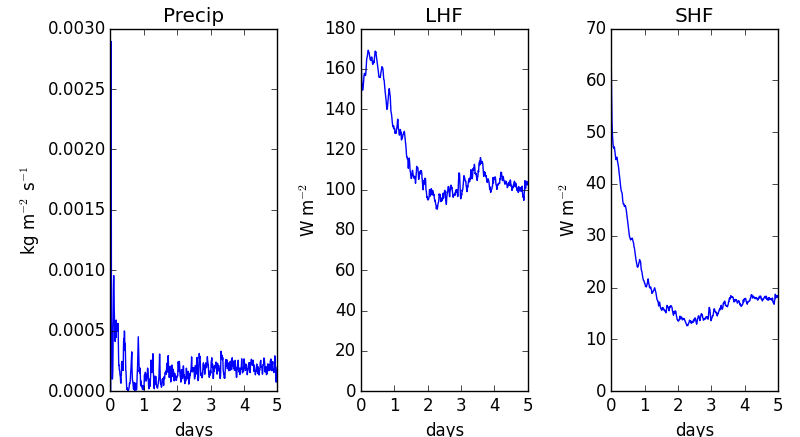
\includegraphics[width=300px]{figures/figure_precip_lhf_shf}
    \caption{Domain averaged precipitation, sensible heat flux (SHF) and latent heat flux (LHF).}
    \label{fig:precip}
\end{figure}

\begin{figure}[hbp!]
    \centering
    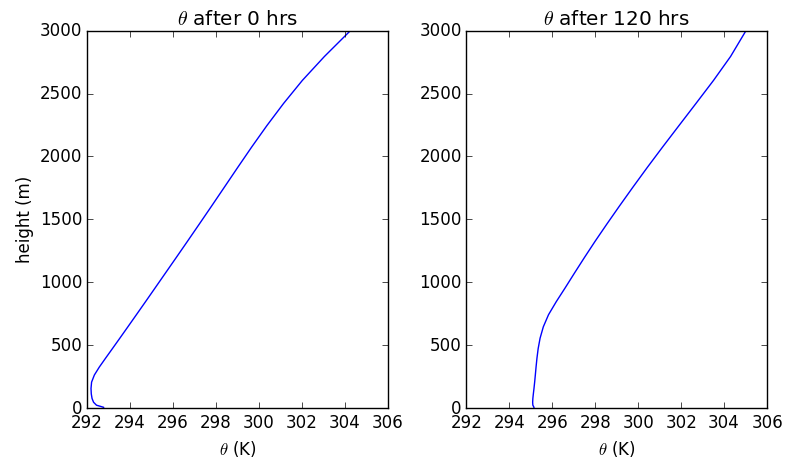
\includegraphics[width=300px]{figures/figure_th0_120}
    \caption{Initial and final $\theta$ profiles.}
    \label{fig:th0}
\end{figure}

\begin{figure}[htp!]
    \centering
    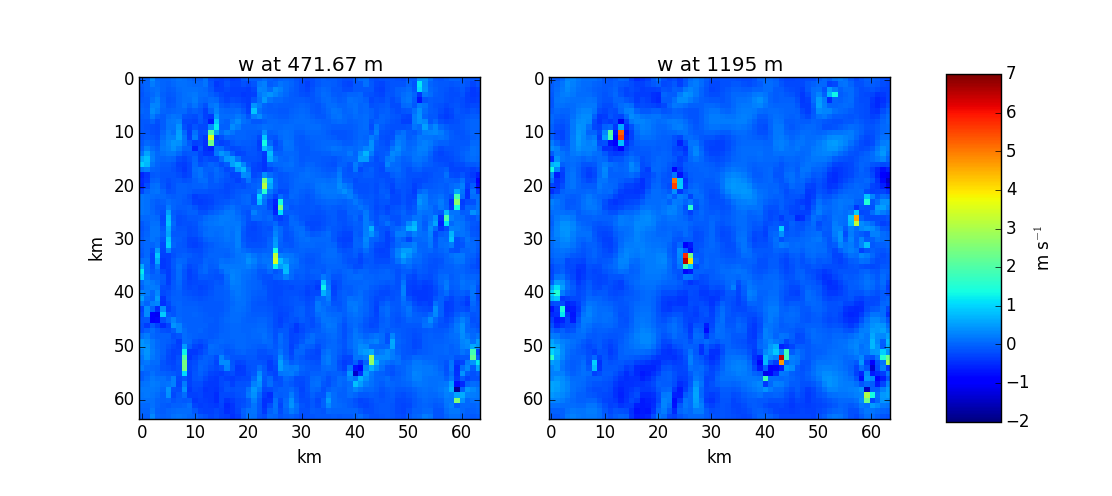
\includegraphics[width=350px]{figures/figure_2d}
    \caption{Final $w$ at 471.67 m and 1195 m.}
    \label{fig:w_final_471}
\end{figure}

\newpage
\subsection{Modules}

The MSc modules have given me a foundation to understand my topic area, from the mathematical
derivations through to the model implementation. Because I did not have a background in meteorology,
I put a lot of effort in to them to make sure that I was up to speed with the relevant maths and
physics and that I could place my research into a wider atmospheric research context. I was pleased
with my results, although I am fully aware that these are only necessary and not sufficient to for
me to make the most of my PhD.

\begin{tabular}{ |l|l|l| }
\hline
\multirow{3}{*}{Autumn} & Atmospheric Physics & 79 \\
  & Fluid Dynamics (with non-assessed practicals) & 94 \\
  & Introduction to Numerical Modelling & 90 \\
\hline
\multirow{3}{*}{Spring}   & Tropical Weather Systems & 82 \\
  & Numerical Modelling of Atmospheres and Oceans & 92 \\
  & Global Circulation of the Atmosphere and Ocean & 86 \\
\hline
\end{tabular}

\section{Future work}

In the short term I will be focussed on running an RCE experiment using the iUM in a low-resolution
configuration, with \SI{1}{km} grid length and a timestep of \SI{60}{s}. The low-resolution will
allow me to perform runs using the Archer short queue, which will greatly speed up the development
time.  The iUM version will be based on Chris Smith's 10.4 branch, and I will keep up-to-date with
developments to this branch as well as feeding back information to Chris and Adrian Hill at the Met
Office. I will also use the diagnostics from this low-resolution run as test input for scripts that
can start to analyse its output.

% A balance moisture budget needs latent heat flux to balance precip.
% A balanced heat budget needs sensible and latent heat balance radiation cooling.
Once the low-resolution runs are working as expected - latent heat flux balances precipitation,
sensible and latent heat flux balance the atmospheric cooling, and the atmosphere stabilizes with
its lowest level having a temperature of \SI{300}{K} - I will increase the resolution up to
\SI{50}{m} grid lengths. At this point I will be in a position to start performing useful
experiments, and will begin experiments with varying wind shear to vary the amount of convective
organization. In conjunction with this, I will start to develop and test diagnostics for determining
the amount of organization present in the experiments. These experiments will form the basis of my
control runs against which I can test parametrization schemes run at different resolutions.

In the longer term (3-6 months), I will begin to investigate how parametrization schemes behave in
the grey-zone when modelling RCE experiments. This will involve varying the resolution across some
grey-zone scales, and also involve seeing how the parametrization copes with convective
organization. The parametrization used will most likely be based on the \cite{plant2008stochastic}
scheme, which should mean that it is scale aware.

During this time I will also produce a preliminary literature review of different convective
parametrization schemes, with a focus on those that are most relevant for my thesis, such as those
that are in some sense scale aware.

This work builds towards my longer term goals of investigating the organizational structure of cloud
fields in a simplified setup. The high-resolution models will allow me to analyse the statistics of
the could field, e.g. calculating the average distance between clouds, working out if clouds are
randomly positioned. This could be coupled with analytical or extremely simplified models of the
cloud spacing to see if these provide physical insight into these processes. The work on cloud field
structure will feed into the parametrization experiments, where I will look into using these results
to vary the parametrization in a way that effectively mimics the changes in the mean flow due to
cloud organization. The literature review will give me a foundation for fitting my work into a
larger context, as well as being useful for writing up my thesis. 

More speculatively, I am also interested in questions surrounding the triggering of larger scale
features by grid-scale disturbances. Another interesting question would be what would happen if a
high-resolution model's grid-scale variability were fed into a lower resolution model as its subgrid
variability, and whether the two models remain in synchrony with each other. These represent
possible directions that my research might take if there is enough time and if there are compelling
reasons for going down one of these routes.

\section{Training record}

\subsection{Scientific courses}
\label{sec:Scientific courses}
In December I went to a course on the UM, which gave me an appreciation of how many things can go
wrong with the model, such as compilation errors, reconfiguration errors and runtime errors, as well
as giving me some pointers on how to fix them. Unfortunately the bulk of the course was focussed on
using UMUI, not Rose, although some time was spent on how to use Rose to run the UM as well.
Although there is a lot of commonality between these two methods of running the UM, it would be nice
if the course had taught us the most up-to-date method as the primary method for running it.

In February I attended a course on MONC (Met Office NERC Cloud model), a new high-resolution model
being developed by the Met Office and EPCC (Edinburgh Parallel Computing Centre) that aims to
reproduce all of the functionality offered by LEM (Large Eddy Model). It is written in modern
Fortran (2003) and designed to scale to thousands of cores efficiently. Although there are some
outstanding issues with its functionality, namely required test cases that have not been properly
tested and bugs in its IO server that affects its diagnostic output, its clean code and scalability
could make it very interesting in the near to medium future.

In May I went to a week long course at ECMWF on the parametrization of subgrid physical processes.
This highly worthwhile course looked at the different physical processes that it is necessary to
parametrize in order to build a working global forecast model, from cloud microphysics, boundary
layer and convective clouds to radiation and land surface processes. It also touched on aspects of
Data Assimilation and the interaction between the dynamics and the subgrid parametrization.

I attended the first ParaCon plenary at the end of June. ParaCon (Parametrized Convection) is a new
project aimed at improving the representation of convection across a range of scales. This was a
great chance to see a new project in my subject area beginning to take shape, and to hear about the
scientific challenges in my field. It was also interesting to hear about the latest developments
with idealized models - the iUM and MONC - at the Met Office.

\label{sec:Training record}
\subsection{Transferable skills}
In January I completed the core classes for ``Preparing to teach''. Attending these courses are a
requirement for demonstrating in the 2\ts{nd} year, something that I would be keen to do to 
build my teaching experience at this level.

As a 1\ts{st} year representative for the Post Graduate Research (PGR) forum, I have attended the
meetings to offer a perspective on the proceedings of the department. I also acted as an
intermediary between the PGR forum and the PhD Visiting Scientist committee, which organized the
visit of Richard Rotunno (a distinguished scientist at NCAR, based in Boulder, Colorado) from the
6\ts{th} to the 10\ts{th} of June. This involved sitting on the Visiting Scientist committee,
deciding how the week should be structured, helping to organize various parts of the week and making
sure that Richard felt welcome and that we as PhD students got the most out of the week. Personally,
I enjoyed meeting him very much and came away with a couple of interesting ideas that I am keen to
follow up on.

I have continued to enjoy going to the departmental and lunchtime seminars, finding out more about
diverse topics such as how snow affects radiation, and how representation of supercooled water in
global models can have a big positive impact on their forecasts. I regularly attend mesogroup,
Jonathan Chui's talk on his parametrization scheme was a recent highlight. PhD group on Wednesday
evenings is also a good chance to see what ideas other PhD students are working on in a less formal
setting. I gave a short 15 minute presentation on one of Richard Rotunno's papers there in May.

\printbibliography[title={References}]

\newpage
\section*{Appendix}

\subsection*{Training record}

\begin{itemize}
  \item RRDP: Intermediate/Advanced \LaTeX\ (4/11/2015)
  \item RRDP: You and your supervisor (11/11/2015)
  \item RRDP: Quality assurance in research (18/11/2015)
  \item RRDP (equivalent): UM Training (16-18/12/2015)
  \item RRDP (equivalent): Preparing to teach: Introduction to teaching and Learning (26/01/2016)
  \item Preparing to teach: Marking and feedback (26/01/2016)
  \item Preparing to teach: Laboratory demonstrating and leading small groups (27/01/2016)
  \item MONC Training course (9-10/2/2016)
  \item RRDP (equivalent): Fairbrother Lecture ``A slippery situation: melting ice in Antarctica`` (4/5/2016)
  \item ECMWF Parametrization of subgrid physical processes (16-20/5/2016)
\end{itemize}

\subsection*{Talks and conferences}

\begin{itemize}
  \item Climate Change 2013: The physical science basis Institute of Physics (2/2014)
  \item Dame Julia Slingo: Taking the planet into uncharted territory: What climate models can tell us about the future (9/2014)
  \item SCENARIO NERC DTP Conference (9/6/2015)
  \item Climate Change in the run-up to the Paris conference: what has Physics got to say? (6/11/2015)
  \item ParaCon Plenary 1 (27-28/6/2016)
\end{itemize}

\end{document}
